%-*- coding: UTF-8 -*-
% report.text
% 机器学习实现KNN算法报告
\documentclass[UTF8]{ctexart}
\usepackage{graphicx}
\usepackage{graphics}
\usepackage{float}
\usepackage[colorlinks,linkcolor=blue]{hyperref}
\usepackage{listings}
\usepackage{xcolor}
\usepackage{geometry}
\usepackage{setspace}
\usepackage{fancyhdr}
\usepackage{subfigure}

\title{机器学习实验报告}
\author{葛松}
\date{\today}

\geometry{a4paper,left=2cm,right=2cm,top=3cm,bottom=2cm}

\pagestyle{fancy}
\fancyhf{}
\rhead{\thepage}
\lhead{\leftmark}

% 代码样式
\lstset{
    frame=L,
    language=Python,
    aboveskip=3mm,
    belowskip=3mm,
    showstringspaces=false,
    columns=flexible,
    basicstyle={\small\ttfamily},
    numbers=left,
    keywordstyle=\color[RGB]{40,40,255}, 
    commentstyle=\itshape\color{orange},
    stringstyle=\color[RGB]{0.58,0,0.82},
    backgroundcolor=\color[RGB]{245,245,244},  
    breaklines=true,
    breakatwhitespace=true,
    tabsize=4,
%   xleftmargin=\parindent,
%   numbersep=5pt,
}

\begin{document}
\thispagestyle{empty}
\begin{figure}[h]
    \centering
    
\includegraphics[width=3in]{asset/华中科技大学.png}
\end{figure}

\begin{center}
    \fangsong
    \zihao{0}课程实验报告
\end{center}



\vspace*{20mm}
\begin{center}
    \zihao{4}\textbf{题目}:\underline{\makebox[15em]{KNN的Python简单实现}}
\end{center}

\vspace*{70mm}

\begin{center}
    \zihao{5}\textbf{课程名称}: \underline{\makebox[15em]{机器学习}}
    
    \zihao{5}\textbf{专业班级}: \underline{\makebox[15em]{CS1703}}

    \zihao{5}\textbf{学\qquad 号}: \underline{\makebox[15em]{U201714668}}
    
    \zihao{5}\textbf{姓\qquad 名}: \underline{\makebox[15em]{葛松}}
    
    \zihao{5}\textbf{指导教师}: \underline{\makebox[15em]{李玉华}}
    
    \zihao{5}\textbf{报告日期}: \underline{\makebox[15em]{\today}}
\end{center}

\vspace*{50mm}

\begin{center}
    \zihao{4}计算机科学与技术学院
\end{center}
\newpage
\thispagestyle{empty}
\tableofcontents
\newpage
\setcounter{page}{1}
\section{实验一}
\subsection{实验目的与要求}
\begin{enumerate}
    \item 理解KNN算法,及其具体实现
    \item 熟悉Python语言的使用
    \item 熟悉图片的处理方法
\end{enumerate}

% \vspace*{5mm}

\subsection{实验内容}
\begin{enumerate}
    \item 动手实现KNN算法,语言限定为 python。数据集使用 MNIST 数据集。
    \item 最终需要实现以下功能
    \begin{itemize}
        \item 输入若干测试图片,输出对应每张图片 k 近邻的图片。
        \item 绘制 knn 算法的训练 misclassification rate 曲线,并做出分析
        \item 可以自由发挥(人脸数据集等等)
    \end{itemize}
\end{enumerate}

% \vspace*{5mm}
\newpage
\subsection{实验方案}
以下将整个实验内容分为以下几个部分逐一介绍
\begin{quote}
    \begin{itemize}
        \item 整体设计
        \item KNN核心算法
        \item 数据集读取
        \item 输出每张图片k临近的图片
        \item 计算misclassification rate并绘图
    \end{itemize}
\end{quote}

\subsubsection{整体设计}
整个实现过程的流程图如下图所示
\begin{figure}[h]
    \centering
    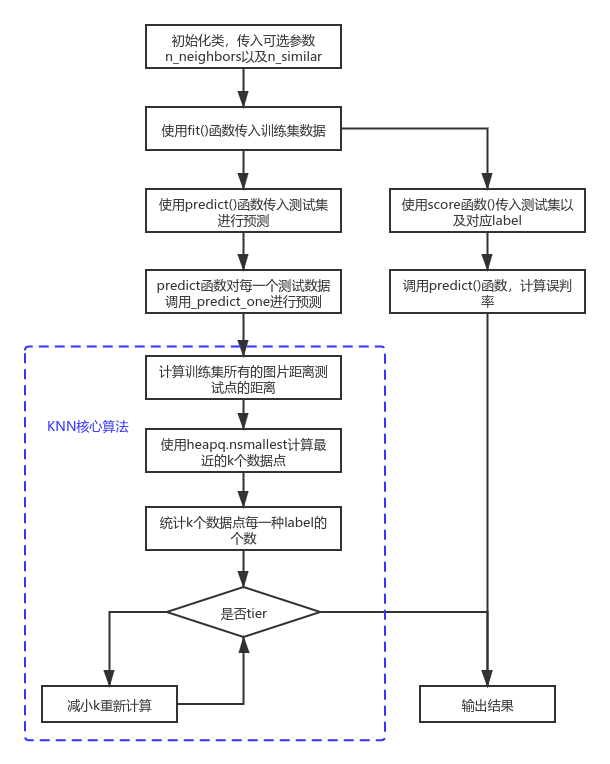
\includegraphics[width=5in]{asset/流程图.png}
    \caption{\lstinline{KNNClassifier}流程图} %最终文档中希望显示的图片标题
    % \label{Fig.main2} %用于文内引用的标签
\end{figure}



该实验中对KNN的实现接口主要参考了\href{https://scikit-learn.org/stable/modules/generated/sklearn.neighbors.KNeighborsClassifier.html}{sklearn中的KNeighborsClassifier}
,将KNN的实现包装在一个类当中,并实现相关方法作为接口开放,类 \lstinline{KNNClassifier}的UML类图如下所示

\begin{figure}[h]
    \centering
    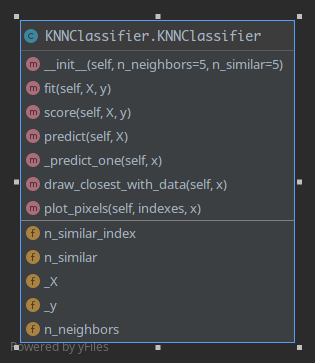
\includegraphics[width=2in]{asset/KNNClassifier_UML.png}
    \caption{\lstinline{KNNClassifier}的UML图} %最终文档中希望显示的图片标题
    % \label{Fig.main2} %用于文内引用的标签
\end{figure}



以下分别介绍\lstinline{KNNClassifier}的属性以及方法

\begin{quote}
    \begin{itemize}
        \item 属性 \lstinline{_X}
        
        用于存放数据集的数据部分,也即图片的numpy表示
        \item 属性 \lstinline{_y}
        
        用于存放数据集的标签部分,也即每一个图片的数字
        \item 属性 \lstinline{n_similar}
        
        用来配置显示最临近的\lstinline{n_similar}个图片的具体数目
        \item 属性 \lstinline{n_similar_index}
        
        保存距离最近的\lstinline{n_similar}个图片在\lstinline{_X}中的下标
    
        \item 方法 \lstinline{fit(X,y)}
    
        用于传入数据,实际上就是将内部的\lstinline{_X}以及\lstinline{_y}设置为对应值
        \item 方法 \lstinline{score(X,y)}
    
        对测试数据\lstinline{X, y}进行打分,输出misclassification rate
        \item 方法 \lstinline{predict(X)}
    
        预测数据\lstinline{X},其中参数\lstinline{X}为numpy数组,表示多个图片
        \item 方法 \lstinline{_predict_one(x)}
    
        与方法\lstinline{predict(X)}配合,用于预测单个图片,其中参数\lstinline{x}为单个图片的numpy表示
        \item 方法 \lstinline{draw_cloest_with_data(x)}
    
        用于绘出与图片\lstinline{x}最接近的\lstinline{n_similar}个图片
        \item 方法 \lstinline{plot_pixels(indexes,x)}
    
        用于和\lstinline{draw_cloest_with_data(x)}配合
    \end{itemize}
\end{quote}

\newpage
\subsubsection{KNN核心算法}

KNN的核心算法主要由\lstinline{_predict_one}来实现,主要代码以及注释如下



\begin{quote}
    \begin{lstlisting}[breaklines, title=\lstinline{_predict_one}方法]
def _predict_one(self, x):
    k = self.n_neighbors
    # 只判断一个,x为728维的数组
    dist_list = list(np.sqrt(((self._X - x) ** 2).sum(axis=1)))
    # (距离,标签,index)三元组,其中index用于定位原来
    dist_list = list(zip(dist_list, self._y, list(x for x in range(0, len(self._X)))))
    # 暂时不考虑第k和第k+1个元素的距离相等的情况
    # 首先通过nsmallest函数获得最近的k个元素
    dist_list = nsmallest(k, dist_list)
    # 再通过np.unique函数返回前k个数据点中每一种标签的数目
    label, counts = np.unique([x[1] for x in dist_list], return_counts=True)
    lable_counts = list(zip(counts, label))
    # 找到数目最多的标签
    lable_counts.sort(reverse=True)
    result = lable_counts[0][1]
    while k > 1 and len(lable_counts) > 1 and lable_counts[0][0] == lable_counts[1][0]:
        # 当最大和第二大相等的时候,需要缩小k,重新进行计算
        if dist_list[k - 1] == lable_counts[0][1]:
            result = lable_counts[1][1]
            break
        elif dist_list[k - 1] == lable_counts[1][1]:
            result = lable_counts[0][1]
            break
        k -= 1
    self.n_similar_index = [x[2] for x in dist_list[:self.n_similar]]  # 选出最近的n的点的index
    return result
    \end{lstlisting}
\end{quote}

\vspace*{2em}


KNN算法主要步骤就是
\begin{quote}
    \begin{itemize}
        \item 计算距离(本次实验采用了欧氏距离)
        \item 排序
        \item 对前k个进行统计
        \item 如果出现个数最多的两个标签数目相等则缩小k值
    \end{itemize}
\end{quote}

其中计算距离通过\lstinline{numpy}的广播机制可以非常方便的计算出来
\begin{quote}
    \begin{lstlisting}[breaklines, frame=tb, numbers=none]
dist_list = list(np.sqrt(((self._X - x) ** 2).sum(axis=1)))
    \end{lstlisting}
\end{quote}

\newpage
排序这里采用了\lstinline{nsmallest}函数,而不是简单的调用\lstinline{sort}方法,由于\lstinline{nsmallest}函数通过构建最小堆的形式来得到
k个最小的元组,当k很小,而整体的个数N很大的时候非常合适,如本次试验中训练集为6000但是k只有1到20,
而对每一种标签的统计也可以通过\lstinline{numpy}的\lstinline{unique()}函数得到
\begin{quote}
    \begin{lstlisting}[breaklines, frame=tb, numbers=none]
# 返回前k个数据点中每一种标签的数目
label, counts = np.unique([x[1] for x in dist_list[:k]], return_counts=True)    
    \end{lstlisting}
\end{quote}

函数末尾的\lstinline{while}循环来解决tier的情况,假设两个标签$A$,$B$的个数相等,且个数在所有的标签当中最大,那么依次从k个元素的末尾取出元素,
直到检查到标签为$A$或者$B$,如果第i个元素检查出$A$,那么说明当k减小到i-1时,$B$的个数将会超过$A$,所以最终结果为$B$,反之亦然,
使用这种方法的目的是为了避免每一次都调用\lstinline{sort}函数导致效率极低

\vspace*{5em}


\subsubsection{数据集读取}
这次实验中的数据集读取直接使用了\lstinline{sklearn}中的\lstinline{fetch_openml}方法
\footnote{在整个试验中仅此一处使用了\lstinline{sklearn},仅仅用于导入数据},可以非常方便的导入\lstinline{numpy}格式的mnist数据。
代码如下所示
\begin{quote}
    \begin{lstlisting}[breaklines]
from sklearn.datasets import fetch_openml
mnist = fetch_openml('mnist_784')
    \end{lstlisting}
\end{quote}
其中\lstinline{mnist}的成员\lstinline{data}即为\lstinline{numpy}格式的70000张手写图片,成员\lstinline{target}即为每一张图片对应的标签


\vspace*{5em}
\subsubsection{输出每张图片k临近的图片}
在\lstinline{_predict_one}方法中排序的同时设置了成员\lstinline{n_similar_index},保存了距离图片\lstinline{x}最近的\lstinline{n_similar}
个图片的下标,进而在方法\lstinline{draw_closest_with_data(x)}使用

方法\lstinline{draw_cloest_with_data}以及\lstinline{plot_pixels}代码如下所示

\begin{quote}
    \begin{lstlisting}[breaklines, title=\lstinline{draw_closest_with_data}方法]
def draw_closest_with_data(self, x):
    """
    x为数据
    """
    result = self._predict_one(x)
    self.plot_pixels(self.n_similar_index, x)
    \end{lstlisting}
\end{quote}


\begin{quote}
    \begin{lstlisting}[breaklines, title=\lstinline{plot_pixels}方法]
def plot_pixels(self, indexes, x):
    """
    x 目标图片的点位数据
    indexes 为最近的n个图片的index
    """
    pixels = np.reshape(x, (28, 28))
    plt.figure(figsize=(2, 2))
    plt.axis('off')
    plt.title(f"Target Image")
    plt.imshow(pixels, cmap='gray')
    count = len(indexes)
    rows = int(count ** 0.5)
    columns = int(count / rows + 1)
    fig = plt.figure(figsize=(columns, rows))
    for i in range(count):
        pixels = np.reshape(self._X[[indexes[i]]], (28, 28))
        ax = fig.add_subplot(rows, columns, i + 1)
        ax.title.set_text(f"No.{indexes[i]}")
        plt.axis('off')
        plt.imshow(pixels, cmap='gray')
    fig.tight_layout()
    plt.show()
    \end{lstlisting}
\end{quote}

输出结果如下图所示
\begin{figure}[h]
    \centering
    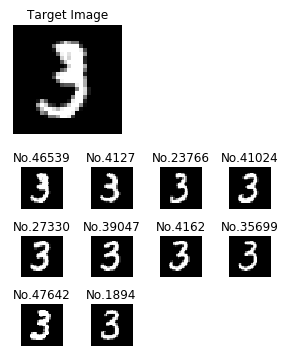
\includegraphics[width=2in]{asset/closest.png}
    \caption{绘制最近的\lstinline{n_similar}个图片} %最终文档中希望显示的图片标题
    % \label{Fig.main2} %用于文内引用的标签
\end{figure}

% \vspace*{10em}
\newpage
\subsubsection{计算 misclassification rate 并绘图}
分别计算k从1到20时的\lstinline{score},也即\lstinline{misclassification rate},再通过\lstinline{matplotlib}进行绘制即可
具体代码如下

\begin{quote}
    \begin{lstlisting}[breaklines, title=计算 misclassification rate]
# 分割测试集和训练集
X = mnist.data
y = mnist.target
X_train,X_test,y_train,y_test = X[:6000], X[6000:7000], y[:6000], y[6000:7000]
data_test = []
data_train = []
for k in range(1, 21):
    # 分别测试k从1到20
    KNN = KNNClassifier(n_neighbors=k)
    KNN.fit(X_train, y_train)
    mis_test = KNN.score(X_test, y_test)
    mis_train = KNN.score(X_train, y_train)
    print(mis_test)
    print(mis_train)
    data_test.append(mis_test)
    data_train.append(mis_train)
# 进行绘制
fig, ax = plt.subplots()
ax.plot([x+1 for x in range(20)], data_test, label='Test', marker='.',markersize=8)
ax.plot([x+1 for x in range(20)], data_train, label='Train', marker='*', markersize=8)
ax.set_ylabel('misclassfication rate', fontsize='medium')
ax.set_xlabel('k', fontsize='medium')
plt.xticks([x for x in range(1,21)], [x for x in range(1,21)])
plt.legend()
plt.show()
    \end{lstlisting}
\end{quote}



\newpage
\subsection{实验结果}
\subsubsection{输出每张图片k临近的图片}
分别测试mnist数据集中的几个图片,输入结果如下




\begin{figure}[h]
    \centering
    \subfigure[测试1]{
        \begin{minipage}[t]{0.4\linewidth}
            \centering
            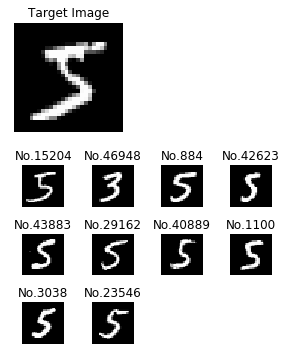
\includegraphics[width=2in]{asset/closest_1.png}
            %\caption{fig1}
        \end{minipage}%
    }%
    \subfigure[测试2]{
        \begin{minipage}[t]{0.4\linewidth}
            \centering
            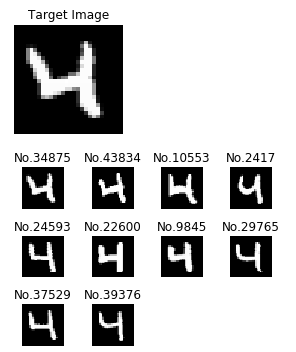
\includegraphics[width=2in]{asset/closest_2.png}
            %\caption{fig2}
        \end{minipage}%
    }%

    
    \subfigure[测试3]{
        \begin{minipage}[t]{0.4\linewidth}
            \centering
            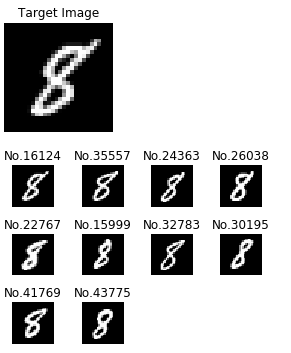
\includegraphics[width=2in]{asset/closest_3.png}
            %\caption{fig1}
        \end{minipage}%
    }%
    \subfigure[测试4]{
        \begin{minipage}[t]{0.4\linewidth}
            \centering
            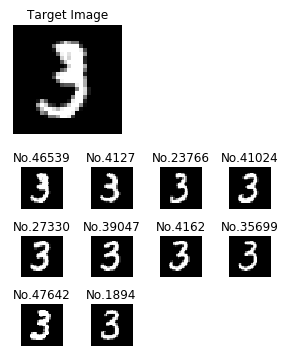
\includegraphics[width=2in]{asset/closest.png}
            %\caption{fig2}
        \end{minipage}%
    }%
    \caption{最近的\lstinline{n_similar}个图片输出}
\end{figure}
可见结果正确

\newpage
\subsubsection{输出misclassification rate曲线}
运行前述代码,由于mnist数据集有70000个并且限于实现代码的运行速度,所以选取了6000张图片作为训练集,1000张图片作为测试集,分别计算k从1到20时,在训练集
以及测试集上的misclassification rate,并绘制曲线
\begin{figure}[h]
    \centering
    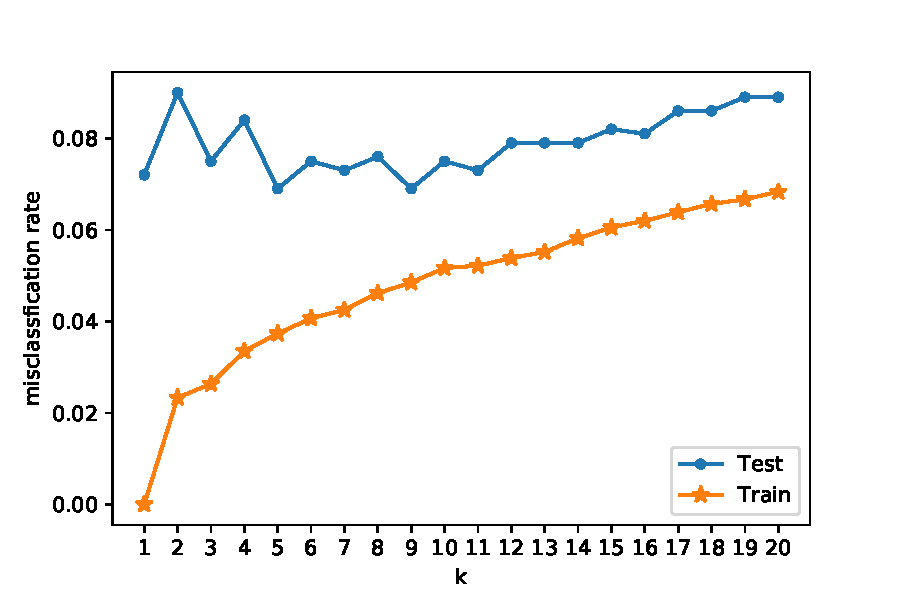
\includegraphics[width=4in]{asset/misclassification.pdf}
    \caption{绘制misclassification rate曲线} %最终文档中希望显示的图片标题
\end{figure}


\zihao{5}\textbf{分析如下:}

在训练集上的错误率随着k值的增大不断增大,由于k越大,考虑的点就越多,受到噪声影响就越大,导致错误率上升。而在测试集上的错误率上下波动,总体呈现先下降
再上升的趋势,在k等于5以及9时达到最小值。综合来看当k等于5时兼顾了准确率以及泛化能力,在1到20中为最优解

\newpage
\subsection{实验总结}
通过本次实验,我对于knn算法有了更加深刻的理解,尤其是对于tier情况的处理,之前仅仅是有个大概的理解,实际上实现起来还是会有很多
细节上的问题,其中最为严重的就是计算速度问题. 在和\lstinline{sklearn}中的KNN实现比较之后,发现我最开始的knn实现速度是真的很慢,于是通过
pycharm的分析功能尝试找出运行速度的瓶颈,最终定位到了三个部分
\begin{quote}
    \begin{itemize}
        \item 距离计算

        由于最开始我是将每一个测试图片与训练集中的每一个向量计算距离,导致速度非常慢,而后利用了\lstinline{numpy}的广播机制,并且由于\lstinline{numpy}的底层并不是使用Python而是C等
        效率更高的语言实现的,所以很大的提高了运行速度
        \item 出现tier情况

        最初对于tier情况就是将k减小然后再一次调用整个过程,而这就导致排序函数被重复调用,之后改为了前文所述的使用\lstinline{while}循环依次检查元素的方法,
        对运行速度也有一定的提升
        \item 找出前k个最近的点
        
        最初是简单的将距离列表\lstinline{dist_list}整体进行排序,再取前k个元素,但是后来注意到取出的元素个数k远小于排序集所包含元素个数,如训练集
        有6000个但是k可能只有1,这就导致效率很低,复杂度为$O(Nlog N)$.而堆排序非常契合这种情况.复杂度仅为$O(klogN)$,在使用堆排序之后又进一步提高了
        运行的效率
    \end{itemize}
\end{quote}
通过优化上述的三个瓶颈,一定程度上提高了运行速度,对于6000大小的训练集且k等于5时,计算大小为1000的测试集需要20秒,但是和sklearn还是有非常大的差距(sklearn的默认实现是0.6秒)
,后来也了解到可以通过使用\lstinline{kd_tree},\lstinline{ball_tree}等特殊数据结构来优化运行速度,但是限于能力和时间还是选择的最原始的方法.

\end{document}